% Three columns (sparse notions | stable dense notions | dependent dense notions) and
% four rows. Arrows are implications. All properties in the same row are equivalent
% on weakly sparse classes. Unlike the original, tree-depth and shrub-depth are left out.
%
% Where model checking is known to be fpt, one centered line below the name of the
% property (\mcdec) cites the algorithm (labeled mc), which assumes a suitable
% decomposition of the input graph to be given, and an algorithm computing such a
% decomposition, or says that this is open (labeled dec). For nowhere denseness both
% are in the same paper, which the line cites once (\mcanddec, labeled mc+dec), and
% for monadic dependence model checking is this paper.
% Bounded stable merge-width coincides with structurally bounded expansion, so its box
% cites the algorithms for the latter: model checking given a decomposition, and the
% efficient reversal of transductions that computes one. The line is gray, including
% the link color, so that it does not distract from the names of the properties.
%
% The bottom line of a box (\ex, gray italics) names example graph classes for which
% this box is the most restrictive property in the hierarchy that they have, each
% followed by a citation (\excite, upright and gray including the link color, like the
% citations of the box itself) of an fpt model checking algorithm for that class.
%
% Boxes are \bw wide and \bh high, the columns are \cs apart (center to center) and
% the rows \rs apart. Each box has three bands: the label on a light gray background,
% the citations on a lighter gray one, and the examples on white. The label band takes
% the top half of the box, and the other two bands a quarter each. A black rule \hz
% below the top of the box separates the label from the citations, and the citations
% end \fz above the bottom, at a gray rule of the same width. The label is centered \tz
% below the top, in the middle of the space above the rule. It is set in a tabular, whose struts align the baselines
% of the one-line labels and center the two-line ones at the same height.
% The baselines of the citations and of the examples are \rb and \eb above the bottom
% of the box. The bands and the rules are drawn in the path picture of the box, which
% comes before its border, so the border lies on top of them. Arrows within a row join
% the boxes at the height of the labels, so that they do not continue the black rules.
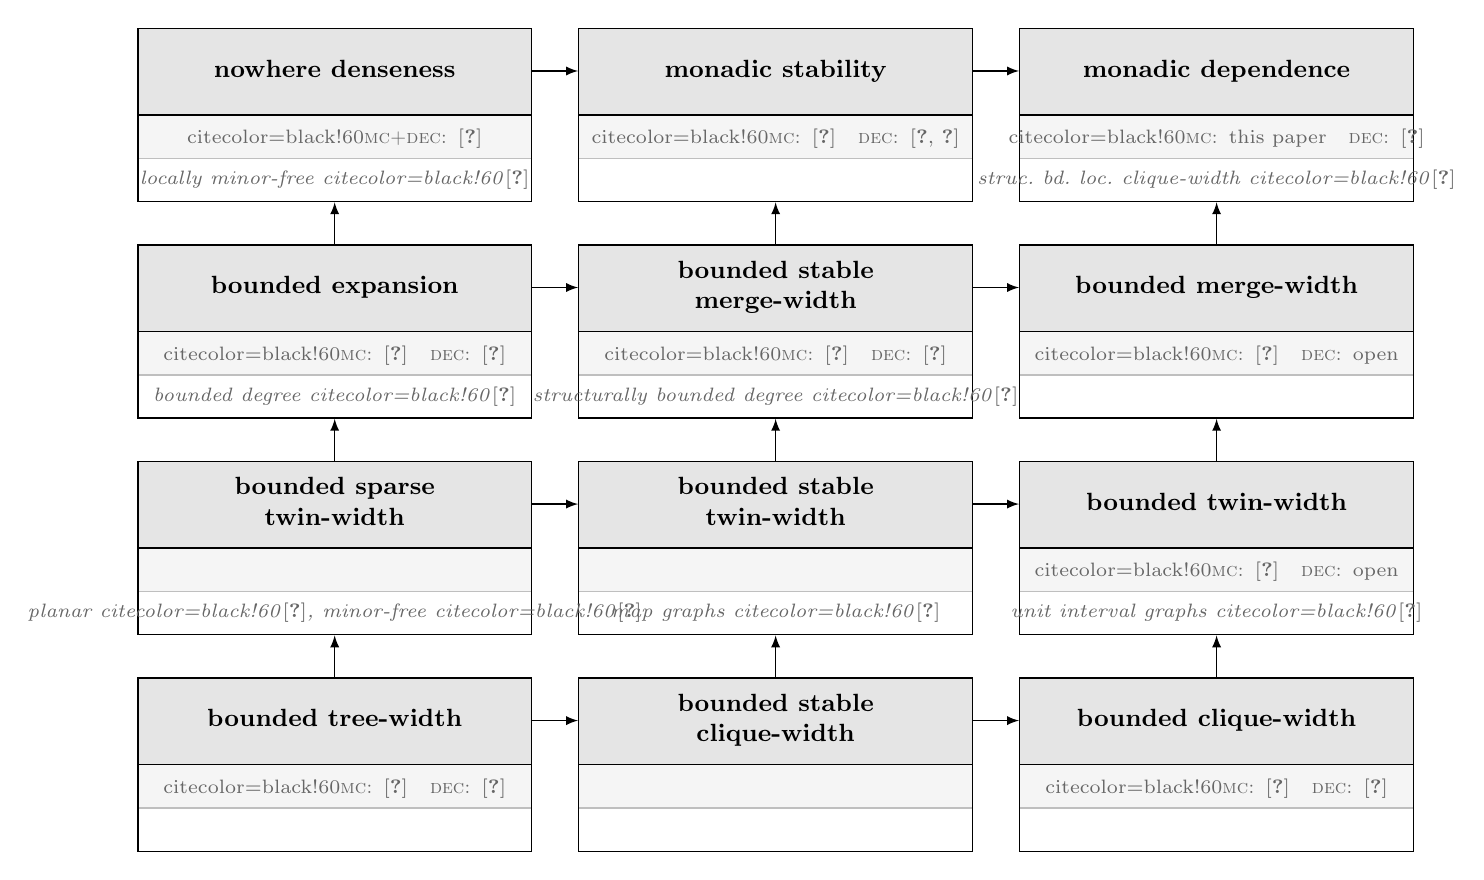
\begin{tikzpicture}[
        prop/.style={draw, line width=0.5pt, minimum width=\bw, minimum height=\bh,
            path picture={\def\pb{path picture bounding box}
                \fill[black!10] (\pb.north west) rectangle ([yshift=-\hz]\pb.north east);
                \fill[black!4] ([yshift=-\hz]\pb.north west) rectangle ([yshift=\fz]\pb.south east);
                \draw[head] ([yshift=-\hz]\pb.north west) -- ([yshift=-\hz]\pb.north east);
                \draw[foot] ([yshift=\fz]\pb.south west) -- ([yshift=\fz]\pb.south east);}},
        proplabel/.style={font=\small\bfseries, inner sep=0pt},
        imp/.style={line width=0.5pt, -latex},
        detail/.style={inner sep=0pt, anchor=base, font=\scriptsize},
        refs/.style={detail, text=black!60,
            execute at begin node={\hypersetup{citecolor=black!60}}},
        example/.style={detail, font=\scriptsize\itshape, text=black!60},
        head/.style={line width=0.5pt},
        foot/.style={line width=0.5pt, black!25},
    ]
    \def\bw{5.0cm}\def\bh{2.2cm}\def\cs{5.6}\def\rs{2.75}
    \def\tz{0.55cm}\def\rb{0.745cm}\def\fz{0.55cm}\def\eb{0.225cm}\def\hz{1.1cm}
    \def\prop#1#2#3{\node[prop] (#1) at (#2) {};
        \node[proplabel] at ([yshift=-\tz]#1.north) {\begin{tabular}{@{}c@{}}#3\end{tabular}};}
    \def\lbl#1{\textsc{#1}}
    \def\mcdec#1#2#3{\node[refs] at ([yshift=\rb]#1.south)
        {\lbl{mc:}\enspace#2\quad\lbl{dec:}\enspace#3};}
    \def\mcanddec#1#2{\node[refs] at ([yshift=\rb]#1.south) {\lbl{mc+dec:}\enspace#2};}
    \def\ex#1#2{\node[example] at ([yshift=\eb]#1.south) {#2};}
    \def\excite#1{{\hypersetup{citecolor=black!60}\textup{\cite{#1}}}}

    % sparse notions
    \prop{nd}{0,0}{nowhere denseness}
    \prop{be}{0,-\rs}{bounded expansion}
    \prop{sptw}{0,-2*\rs}{bounded sparse\\twin-width}
    \prop{trw}{0,-3*\rs}{bounded tree-width}

    % stable dense notions
    \prop{ms}{\cs,0}{monadic stability}
    \prop{smw}{\cs,-\rs}{bounded stable\\merge-width}
    \prop{stw}{\cs,-2*\rs}{bounded stable\\twin-width}
    \prop{scw}{\cs,-3*\rs}{bounded stable\\clique-width}

    % dependent dense notions
    \prop{md}{2*\cs,0}{monadic dependence}
    \prop{mw}{2*\cs,-\rs}{bounded merge-width}
    \prop{tww}{2*\cs,-2*\rs}{bounded twin-width}
    \prop{cw}{2*\cs,-3*\rs}{bounded clique-width}

    % fpt model checking, and computing the decompositions it needs
    \mcanddec{nd}{\cite{gks}}
    \mcdec{be}{\cite{DvorakKT13-journal}}{\cite{grad-and-bounded-expansion-Nesetril}}
    \mcdec{trw}{\cite{courcelle1990monadic}}{\cite{minorsXIII}}
    \mcdec{ms}{\cite{ms-mc1}}{\cite{flippers,ms-mc2}}
    \mcdec{md}{this paper}{\cite{md-abmw}}
    \mcdec{smw}{\cite{lsd-journal}}{\cite{dreier2026efficient}}
    \mcdec{mw}{\cite{mw-stoc}}{open}
    \mcdec{tww}{\cite{tww1}}{open}
    \mcdec{cw}{\cite{courcelle2000linear}}{\cite{OumSeymour-approximating}}

    % example graph classes
    \ex{sptw}{planar~\excite{frick2001deciding}, minor-free~\excite{flum2001fixed}}
    \ex{be}{bounded degree~\excite{seese_1996}}
    \ex{smw}{structurally bounded degree~\excite{new-perspective-journal}}
    \ex{stw}{map graphs~\excite{eickmeyer2017map}}
    \ex{tww}{unit interval graphs~\excite{ganian2015fo}}
    \ex{md}{struc.\ bd.\ loc.\ clique-width~\excite{DBLP:conf/lics/BonnetDGKMST22}}
    \ex{nd}{locally minor-free~\excite{dawar2007locally}}

    % implications within the columns
    \foreach \a/\b in {trw/sptw, sptw/be, be/nd,
                       scw/stw, stw/smw, smw/ms,
                       cw/tww, tww/mw, mw/md}
        \draw[imp] (\a) -- (\b);

    % implications within the rows
    \foreach \a/\b in {nd/ms, ms/md, be/smw, smw/mw, sptw/stw, stw/tww,
                       trw/scw, scw/cw}
        \draw[imp] ([yshift=-\tz]\a.north east) -- ([yshift=-\tz]\b.north west);
\end{tikzpicture}%
